\documentclass[12pt, twoside]{article}
\usepackage[letterpaper, margin=1in, headsep=0.5in]{geometry}
\usepackage[english]{babel}
\usepackage[utf8]{inputenc}
\usepackage{amsmath}
\usepackage{amsfonts}
\usepackage{amssymb}
\usepackage{tikz}
\usetikzlibrary{quotes, angles}
\usepackage{graphicx}
\usepackage{enumitem}
\usepackage{multicol}

\newif\ifmeta
\metatrue %print standards and topics tags

\title{Regents Geometry}
\author{Chris Huson}
\date{January 2022}

\usepackage{fancyhdr}
\pagestyle{fancy}
\fancyhf{}
\renewcommand{\headrulewidth}{0pt} % disable the underline of the header
\raggedbottom

\fancyhead[LE]{\thepage}
\fancyhead[RO]{\thepage \\ Name: \hspace{4cm} \,\\}
\fancyhead[LO]{BECA / Dr. Huson / Geometry 6 Trigonometry}

\begin{document}
\subsubsection*{6.10 Do Now Quiz: Calculator use \hfill CCSS.HSG.SRT.C.8}
\begin{enumerate}
  \item Express the result to the nearest thousandth. Angle measures are in degrees. \vspace{.25cm}
  \begin{multicols}{2}
    \begin{enumerate}
      \item $\displaystyle \tan 33^\circ = $ \vspace{1cm}
      \item $\displaystyle \tan 81^\circ = $
    \end{enumerate}
  \end{multicols} \vspace{1cm}
  
  \item Find the tangent of each radian angle measure. Round to the nearest thousandth. \vspace{.25cm}
  \begin{multicols}{2}
    \begin{enumerate}
      \item $\displaystyle \tan 1.1 = $ \vspace{1cm}
      \item $\displaystyle \tan \frac{\pi}{5} = $
    \end{enumerate}
  \end{multicols} \vspace{1cm}

\item Find each angle measure, to the nearest whole degree.\vspace{.25cm}
\begin{multicols}{2}
  \begin{enumerate}
    \item $\displaystyle \tan^{-1} (\frac{7}{4}) = $ \vspace{1cm}
    \item $\tan^{-1} (0.75) =$
  \end{enumerate}
\end{multicols} \vspace{1cm}

\item Convert between radians and degrees. Leave radians in terms of $\pi$.\vspace{.25cm}
\begin{multicols}{2}
  \begin{enumerate}
    \item $60^\circ = $ \vspace{1cm}
    \item $\displaystyle \frac{\pi}{8} =$
  \end{enumerate}
\end{multicols} \vspace{1cm}

\item Find the value, rounding to the nearest hundredth.\\[0.25cm]
$AB=\sqrt{(-7.7)^2+(26.4)^2}$
\vspace{2.5cm}

\item Mark and label the diagram to reflect the equation:
\begin{multicols*}{2}
  $\displaystyle \tan 41^\circ = \frac{12}{14}$\\
  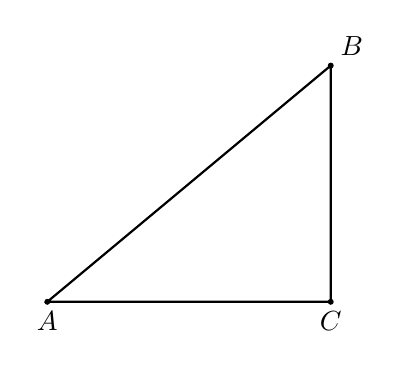
\begin{tikzpicture}[scale=0.6]
    \draw [thick](0,0)--(6,0)--(6,5)--cycle;
    \draw [fill] (0,0) circle [radius=0.05] node[below]{$A$};
    \draw [fill] (6,0) circle [radius=0.05] node[below]{$C$};
    \draw [fill] (6,5) circle [radius=0.05] node[above right]{$B$};
  \end{tikzpicture}
%\end{flushright}
\end{multicols*}


\newpage
\item Solve each equation, rounding to the nearest tenth.
  \begin{enumerate}
  \item $\displaystyle \tan 53^\circ = \frac{x}{11}$ \vspace{5cm}
  \item $\displaystyle \tan 47^\circ = \frac{19}{x}$ \vspace{4cm}
  \item $\displaystyle \tan \theta = \frac{5.7}{4.4}$ \vspace{4cm}
  \item $41=\sqrt{x^2+40^2}$
\end{enumerate}  

\end{enumerate}
\end{document}
